\documentclass[11pt,a4paper]{article}
\usepackage{fontspec}
\setmainfont{TeX Gyre Pagella}
\newfontfamily\headfont{Inter}[UprightFont=*-ExtraBold,BoldFont=*-ExtraBold,Extension=.otf,Path=/usr/share/fonts/opentype/inter/]
\usepackage[a4paper,margin=2.3cm]{geometry}
\usepackage{graphicx,booktabs,float,caption,array,xcolor,longtable}
\usepackage[hidelinks]{hyperref}
\usepackage{titlesec}
\usepackage[round]{natbib}
\usepackage{setspace}
\setstretch{1.05}
\renewcommand{\topfraction}{0.9}
\renewcommand{\bottomfraction}{0.8}
\renewcommand{\textfraction}{0.1}
\renewcommand{\floatpagefraction}{0.75}
\setlength{\parindent}{0pt}
\setlength{\parskip}{0.55em}
\titleformat{\section}{\headfont\Large}{\thesection}{0.8em}{}
\titleformat{\subsection}{\headfont\large}{\thesubsection}{0.8em}{}
\captionsetup{font=small,labelfont=bf}
\urlstyle{same}
\hypersetup{pdftitle={Where the World's Islands Are},pdfauthor={Tristan Hotham}}

\begin{document}
\begin{center}
{\Large\bfseries Where the World's Islands Are\par}
\vspace{0.4em}
{\large Counting, measuring and peopling every island in the GSHHG shoreline\par}
\vspace{1.2em}
{\large Tristan Hotham\par}
\vspace{0.3em}
{\small Independent researcher\\
ORCID: 0000-0003-4931-9349\\
DOI: \href{https://doi.org/10.5281/zenodo.23848301}{https://doi.org/10.5281/zenodo.23848301}\par}
\vspace{0.8em}
2026
\end{center}

\begin{quote}
\small
\begin{center}\textbf{Abstract}\end{center}
How many islands are there, who has them, and how many people live on them? I count every island in the full-resolution GSHHG shoreline, give each a country from Natural Earth and a population from WorldPop's 2025 estimate at about 1 km, and test how far the count depends on the map. GSHHG draws 181,588 islands: 179,823 at sea, 1,437 in lakes and rivers and 328 around Antarctica. 51.8\% are smaller than 0.1 km$^2$; 23,150 are 1 km$^2$ or more, 296 are 1,000 km$^2$ or more. Below 1 km$^2$ the total depends on resolution: the five GSHHG resolutions give 762 to 181,588 islands and Natural Earth 10m gives 9,628, while counts of islands of 1 km$^2$ or more agree within 378 across the three finest GSHHG versions. Canada has the most islands on every threshold (4,048 of 1 km$^2$ or more). Islands cover 6.6\% of the world's land and hold 841 million people, 10.3\% of the world's population; Java, Honshu and Great Britain alone hold 38\% of them. Among islands of 100 km$^2$ or more the most crowded is Xiamen Island (18,787 people per km$^2$); 77 islands of 1,000 km$^2$ or more have no one in the population grid. The largest island in a lake on an island is Glover Island in Newfoundland (163 km$^2$). The results depend on decisions made by the shoreline (what is joined, what is split) and on a modelled population, which I set out.

\textbf{Keywords:} islands; shorelines; GSHHG; WorldPop; population; coastline paradox; Natural Earth; geography
\end{quote}

\section{Introduction}
Island counts are a staple of national pride and of quiz books. Sweden counts 267,570 islands in its national map, Norway and Finland quote figures in the tens of thousands, and Indonesia has repeatedly revised the number of its islands. These figures are not comparable, because the number of islands depends on the definition of an island and, more than anything, on the scale of the map: the coastline paradox applies to islands as much as to coastlines \citep{mandelbrot}. A finer map does not only draw the same islands more precisely; it draws new ones.

This study takes a different route. Rather than seek the true number, it counts everything in one open, consistent, global shoreline, GSHHG \citep{gshhg}, and reports how the count changes with resolution. It then asks who holds the islands, how large they are, and how many people live on them, using WorldPop's gridded population for 2025 \citep{worldpop}. An interactive map accompanies the paper (\url{https://maps.tristanhotham.com/world-islands/}).

\section{Data}
\textbf{Shorelines.} GSHHG 2.3 \citep{gshhg}, in the five resolutions packaged for the basemap Python library (crude, low, intermediate, high and full). Its polygons are hierarchical: level 1 is land bounded by the sea, level 2 a lake, level 3 an island in a lake; Antarctica and the islands in its ice front are kept apart at level 5 in this package. Each polygon carries GSHHG's own area. Polygons cut at the date line are stored in two pieces with a shared identifier.

\textbf{Population.} WorldPop Global 2, release 2024B, constrained estimate for 2025 at 30 arc seconds \citep{worldpop}. The constrained model distributes census-based totals only into grid cells with detected buildings. I used a public re-tiling of this raster on GitHub (world-population-3d, MIT licence), which keeps every cell with 3 or more people in 957 tiles of 5 degrees, with log-quantised counts (relative error under 0.05\%). It holds 31,873,615 cells and 8,187.6 million people. Dropping cells under 3 people loses a negligible share of the total.

\textbf{Countries and names.} Natural Earth 10m admin-0 countries, physical labels (island polygons and points), land and minor islands, and populated places \citep{naturalearth}.

\begin{table}[tbp]\centering\small\caption{Sources, what was used and licences.}\label{tab:sources}\begin{tabular}{>{\raggedright\arraybackslash}p{3.2cm}>{\raggedright\arraybackslash}p{7.6cm}>{\raggedright\arraybackslash}p{2.6cm}}\toprule Source & Used & Licence\\\midrule
GSHHG 2.3, full & 181,588 islands (179,823 sea, 1,437 lake, 328 Antarctic); 6,658 lakes & LGPL-3.0\\
GSHHG 2.3, other resolutions & Island counts (crude, low, intermediate, high) & LGPL-3.0\\
WorldPop Global 2, 2025 & 31,873,615.0 populated cells at 30 arc seconds & CC BY 4.0\\
Natural Earth 10m & Countries, island names, land and minor islands, places & Public domain\\
\bottomrule\end{tabular}\end{table}

\section{Methods}
\subsection{What counts as an island}
Every level-1 polygon other than the five continents (Eurasia, Africa, North America, South America and Australia, each over 5 million km$^2$) is a sea island. Every level-3 polygon is an island in a lake or river; 412 of these lie in lakes that GSHHG flags as river lakes. Antarctic level-5 polygons other than the continent are counted as Antarctic islands. Date-line pieces are joined. Area is GSHHG's area within the coastline, including any lakes. GSHHG judges what is joined and what is separate, and I keep its judgement: Manhattan and Mumbai's Salsette Island are joined to the mainland, Samosir is joined to the shore of Lake Toba, the Island of Montreal and Laval form one island, and the Brodeur Peninsula is cut off from Baffin Island.

\subsection{Countries, regions and names}
Each island takes the Natural Earth country under its representative point, or the nearest one when the point lies outside the Natural Earth coast (most small islands). For the 296 islands of 1,000 km$^2$ or more I measured the geodesic area of each country's share and assigned the island to the largest. Regions follow Natural Earth's continent and subregion fields, with geographic exceptions (Hawaii, Easter Island and New Guinea to Oceania; the French and Dutch Caribbean to the Caribbean; R\'eunion and Mayotte to Africa; Asian Russia to Asia; the French Southern Lands, Heard Island and South Georgia to Antarctica and the far south). Names come from Natural Earth's physical labels; the larger islands it leaves unnamed were named by hand from position, size and largest town, and doubtful ones were left unnamed.

\subsection{Population}
For each tile, land polygons were burned into a grid aligned with the population cells, continents and sea islands first, lakes removed, then islands in lakes, so that each cell takes the polygon under its centre. Cells whose centre lies in the sea or a lake (coastal cells) were given to a polygon touching the cell, which keeps thin islands and atolls, or else to the nearest land cell within two cells. 51.5 million people were placed by touch and 3.8 million by distance; 1.5 million could not be placed. Each cell was also given a Natural Earth country, for national totals.

\section{Results}
\subsection{How many islands}
GSHHG at full resolution has 181,588 islands (Figure~\ref{fig:map}). The distribution is extremely skewed (Figure~\ref{fig:sizes}): 93,998 islands (51.8\%) are under 0.1 km$^2$, 23,150 are 1 km$^2$ or more, 6,341 are 10 km$^2$ or more, 1,512 are 100 km$^2$ or more, 296 are 1,000 km$^2$ or more and 18 exceed 100,000 km$^2$. The smallest island in the data is 177 m$^2$. Islands under 1 km$^2$ make up 87.3\% of the count but 0.2\% of island land. The ten largest islands hold 60.6\% of island land and Greenland alone 21.4\%. In all, islands cover 9.9 million km$^2$, 6.6\% of land.

\begin{figure}[tbp]\centering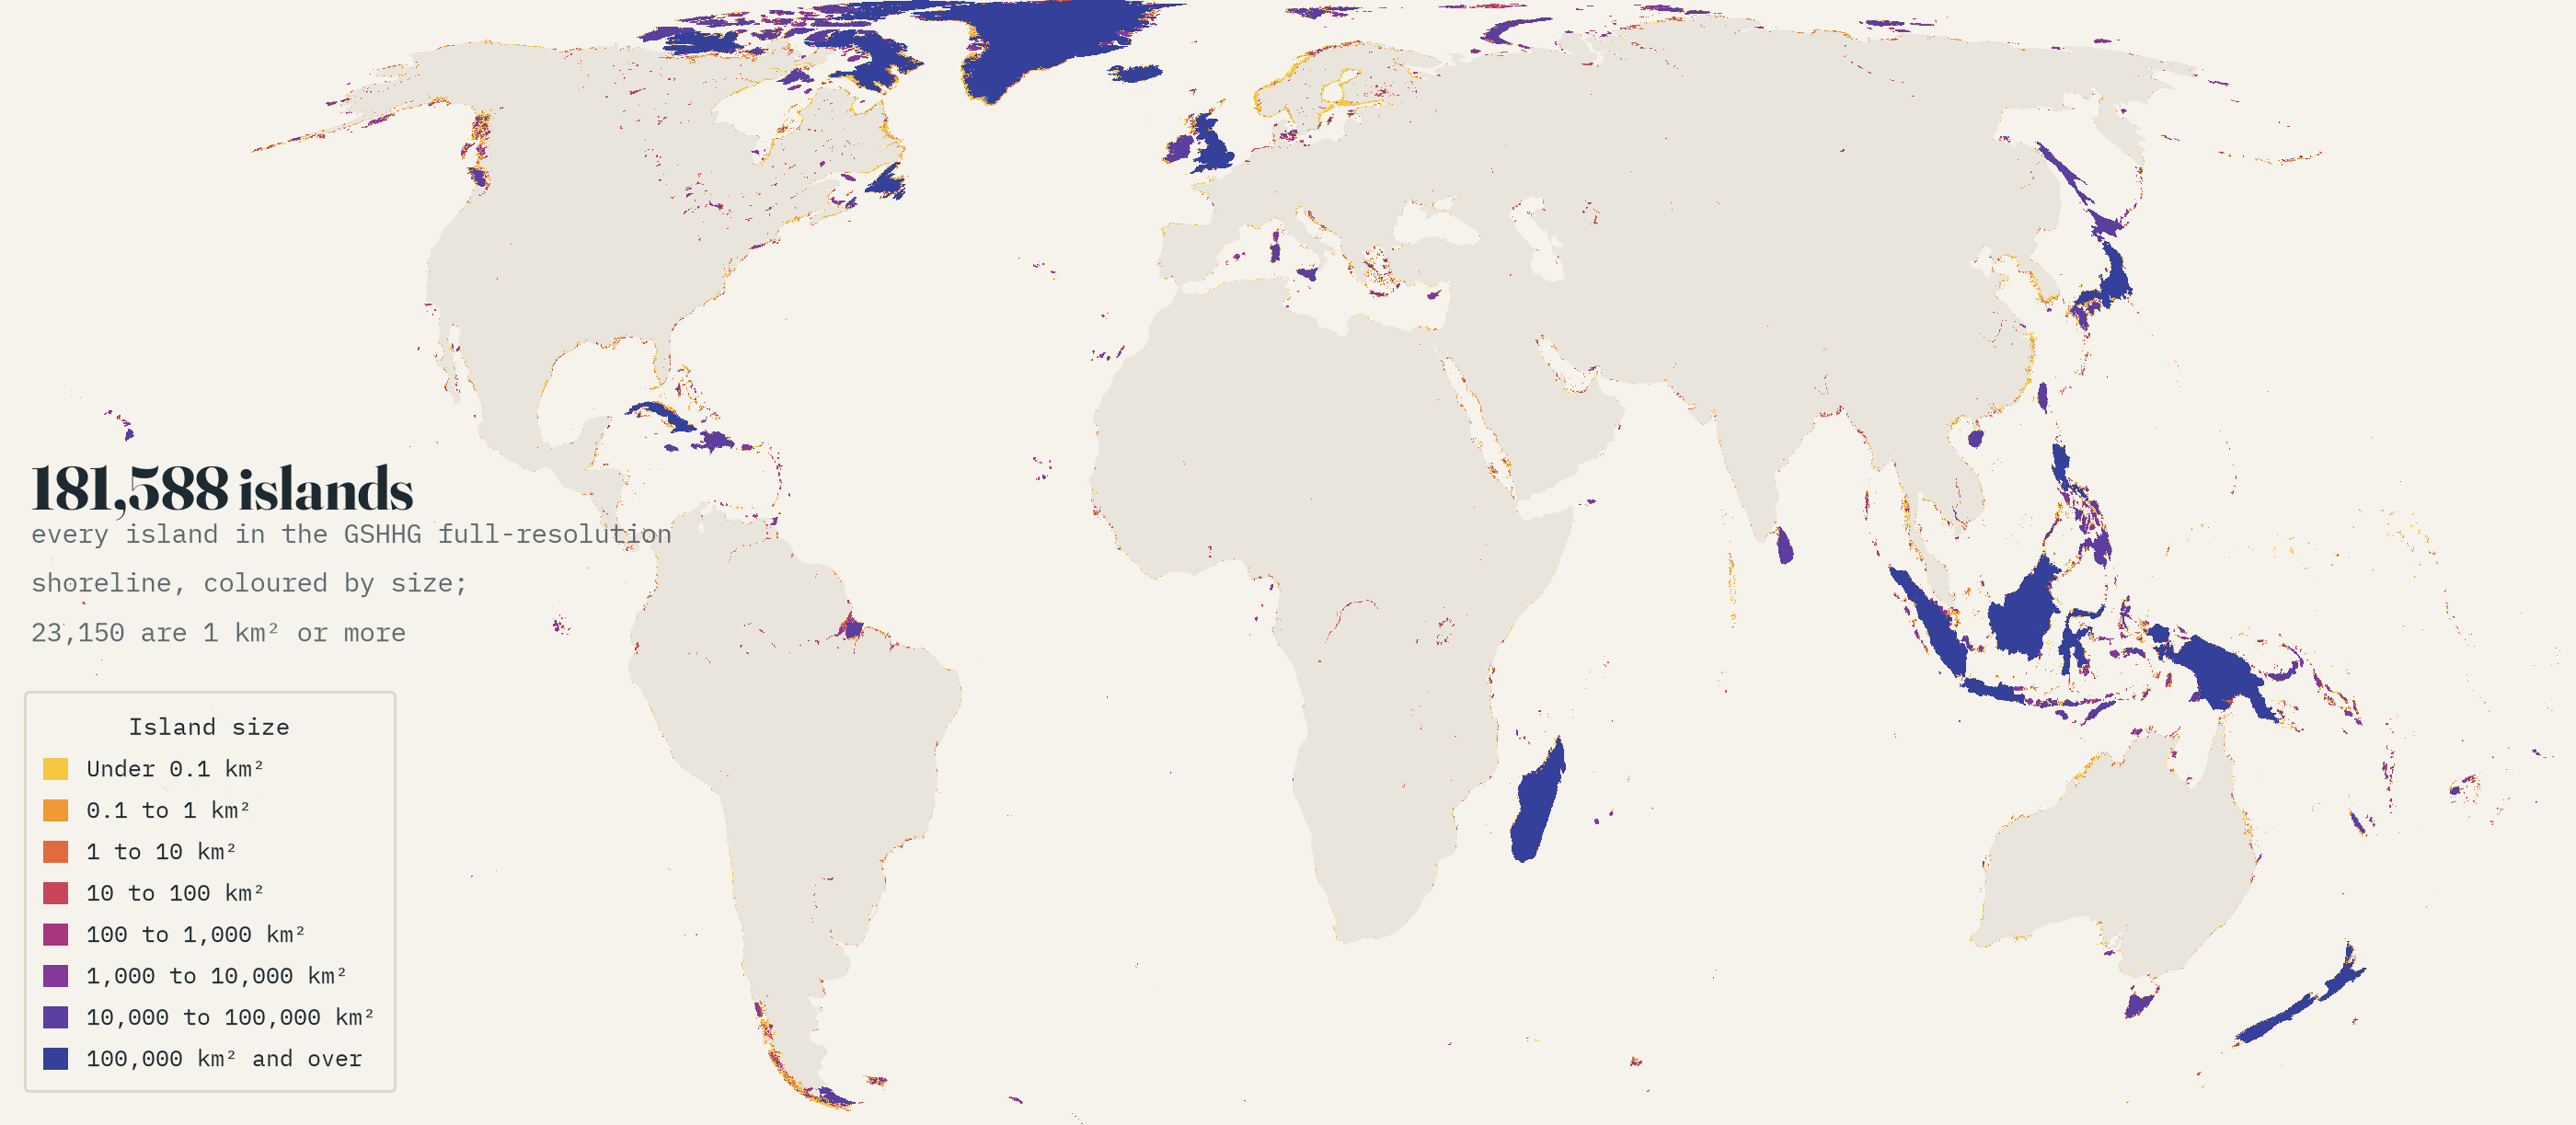
\includegraphics[width=\textwidth]{f_map_world.png}
\caption{Every island in the GSHHG full-resolution shoreline, coloured by size class, in the Equal Earth projection. Tiny islands are drawn as one pixel.}\label{fig:map}\end{figure}

\begin{figure}[tbp]\centering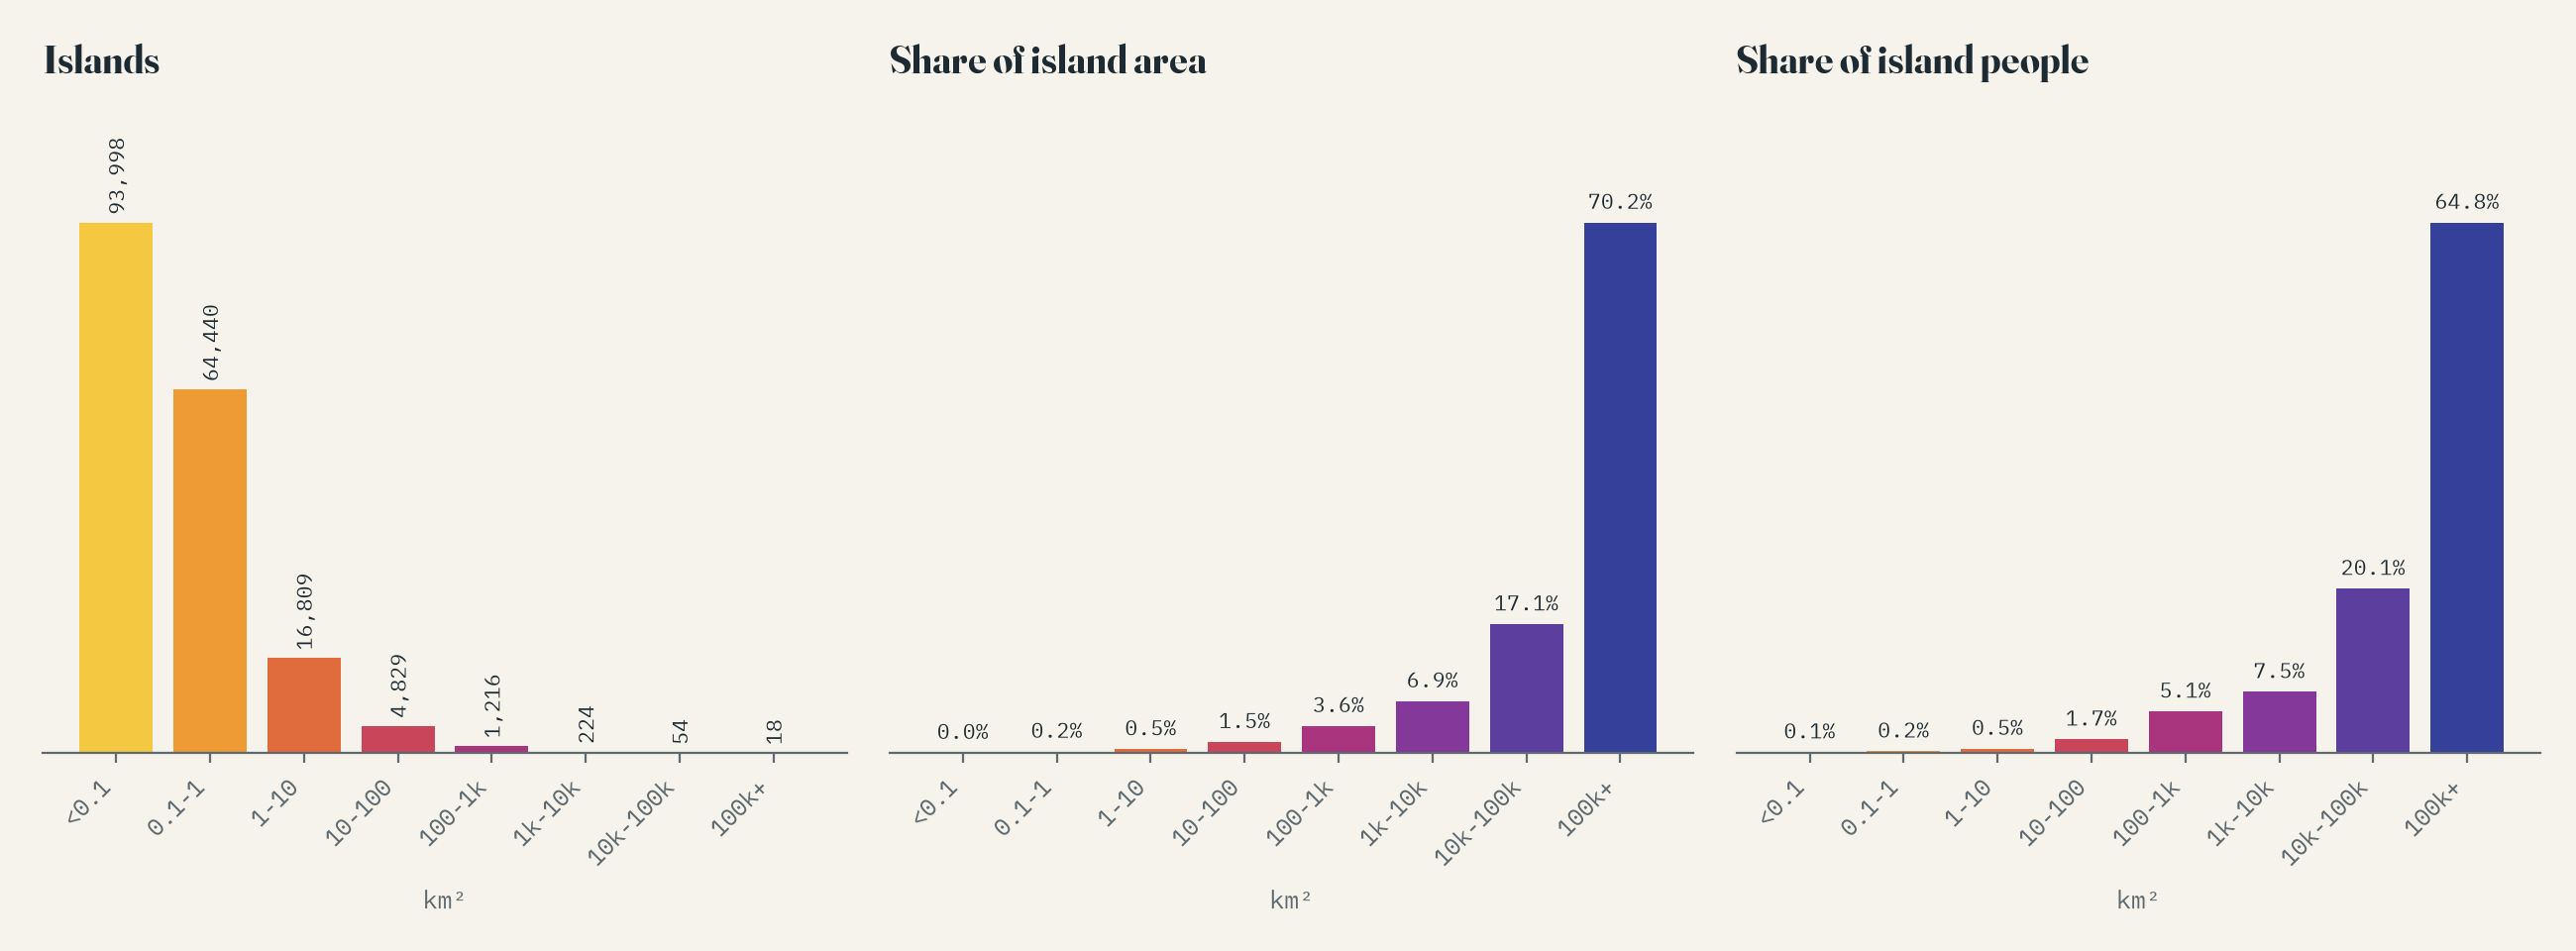
\includegraphics[width=\textwidth]{f_sizes.png}
\caption{Islands by size class: number, share of island land and share of the people living on islands.}\label{fig:sizes}\end{figure}

\subsection{The count depends on the map}
Table~\ref{tab:res} and Figure~\ref{fig:res} compare the five GSHHG resolutions and Natural Earth 10m. The total rises from 762 islands at crude resolution to 181,588 at full, a factor of 238, and full resolution has 18.9 times as many islands as Natural Earth 10m. Each coarser version drops islands below its own resolution (the smallest island at crude resolution is 12 km$^2$). Counts of islands of 1 km$^2$ or more, by contrast, are stable among the three finest GSHHG resolutions (22,772, 23,146, 23,150); Natural Earth has 7,478. For any comparison of countries or regions, I therefore prefer counts at 1 km$^2$ or more. Within a single view of the map the effect is plain: the archipelagos between Stockholm and Turku alone hold 12,849 GSHHG islands, of which 444 are 1 km$^2$ or more (Figure~\ref{fig:baltic}).

\begin{table}[tbp]\centering\small\caption{Islands by map and resolution, all sizes and at or above each area (km$^2$).}\label{tab:res}\begin{tabular}{lrrrrrr}\toprule Map & All & 0.1+ & 1+ & 10+ & 100+ & 1,000+\\\midrule
Natural Earth 10m & 9,628 & 8,544 & 7,478 & 4,309 & 1,464 & 310\\
GSHHG crude & 762 & 762 & 762 & 762 & 730 & 284\\
GSHHG low & 6,242 & 6,242 & 6,242 & 5,257 & 1,502 & 296\\
GSHHG intermediate & 34,392 & 34,392 & 22,772 & 6,339 & 1,512 & 296\\
GSHHG high & 146,510 & 87,309 & 23,146 & 6,340 & 1,512 & 296\\
GSHHG full & 181,588 & 87,590 & 23,150 & 6,341 & 1,512 & 296\\
\bottomrule\end{tabular}\end{table}

\begin{figure}[tbp]\centering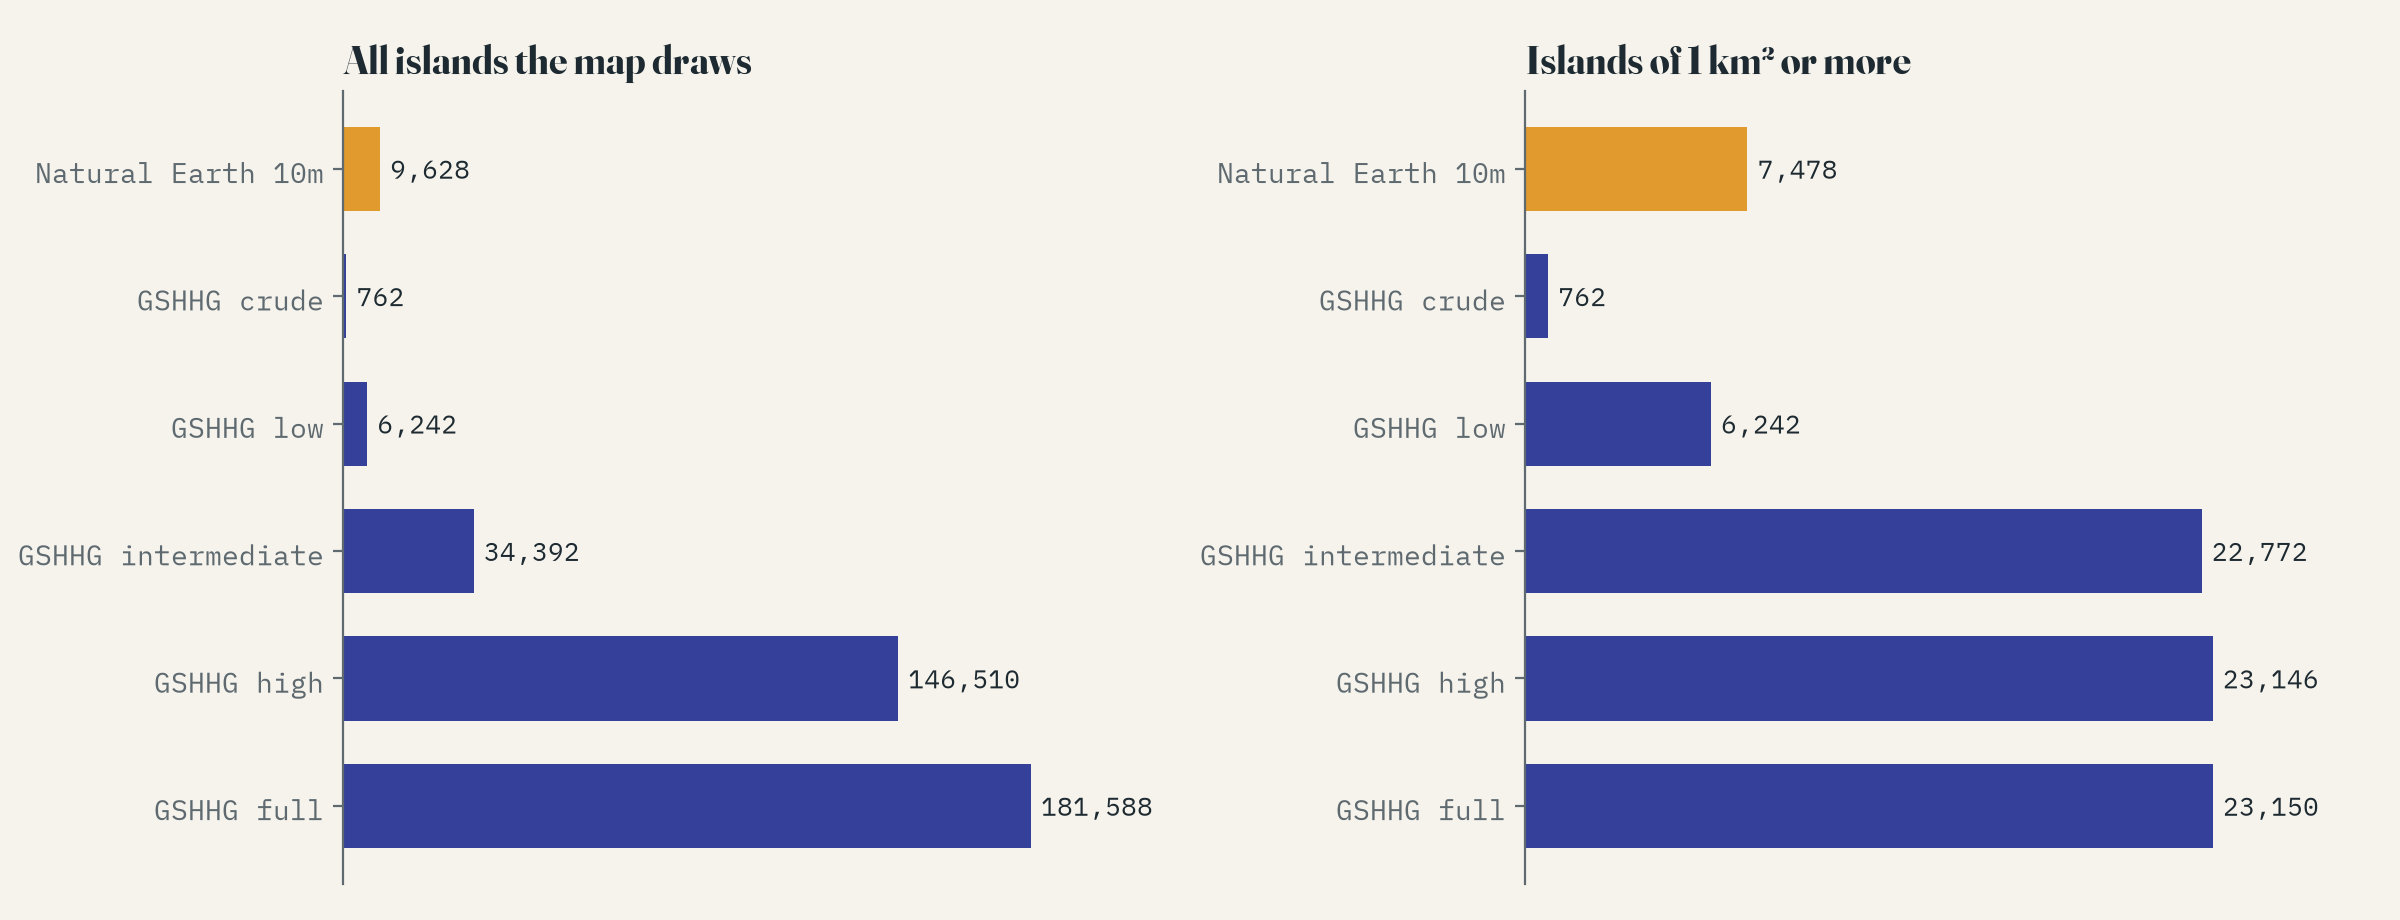
\includegraphics[width=\textwidth]{f_resolutions.png}
\caption{Islands drawn by Natural Earth 10m and by each GSHHG resolution: all sizes and 1 km$^2$ or more.}\label{fig:res}\end{figure}

\begin{figure}[tbp]\centering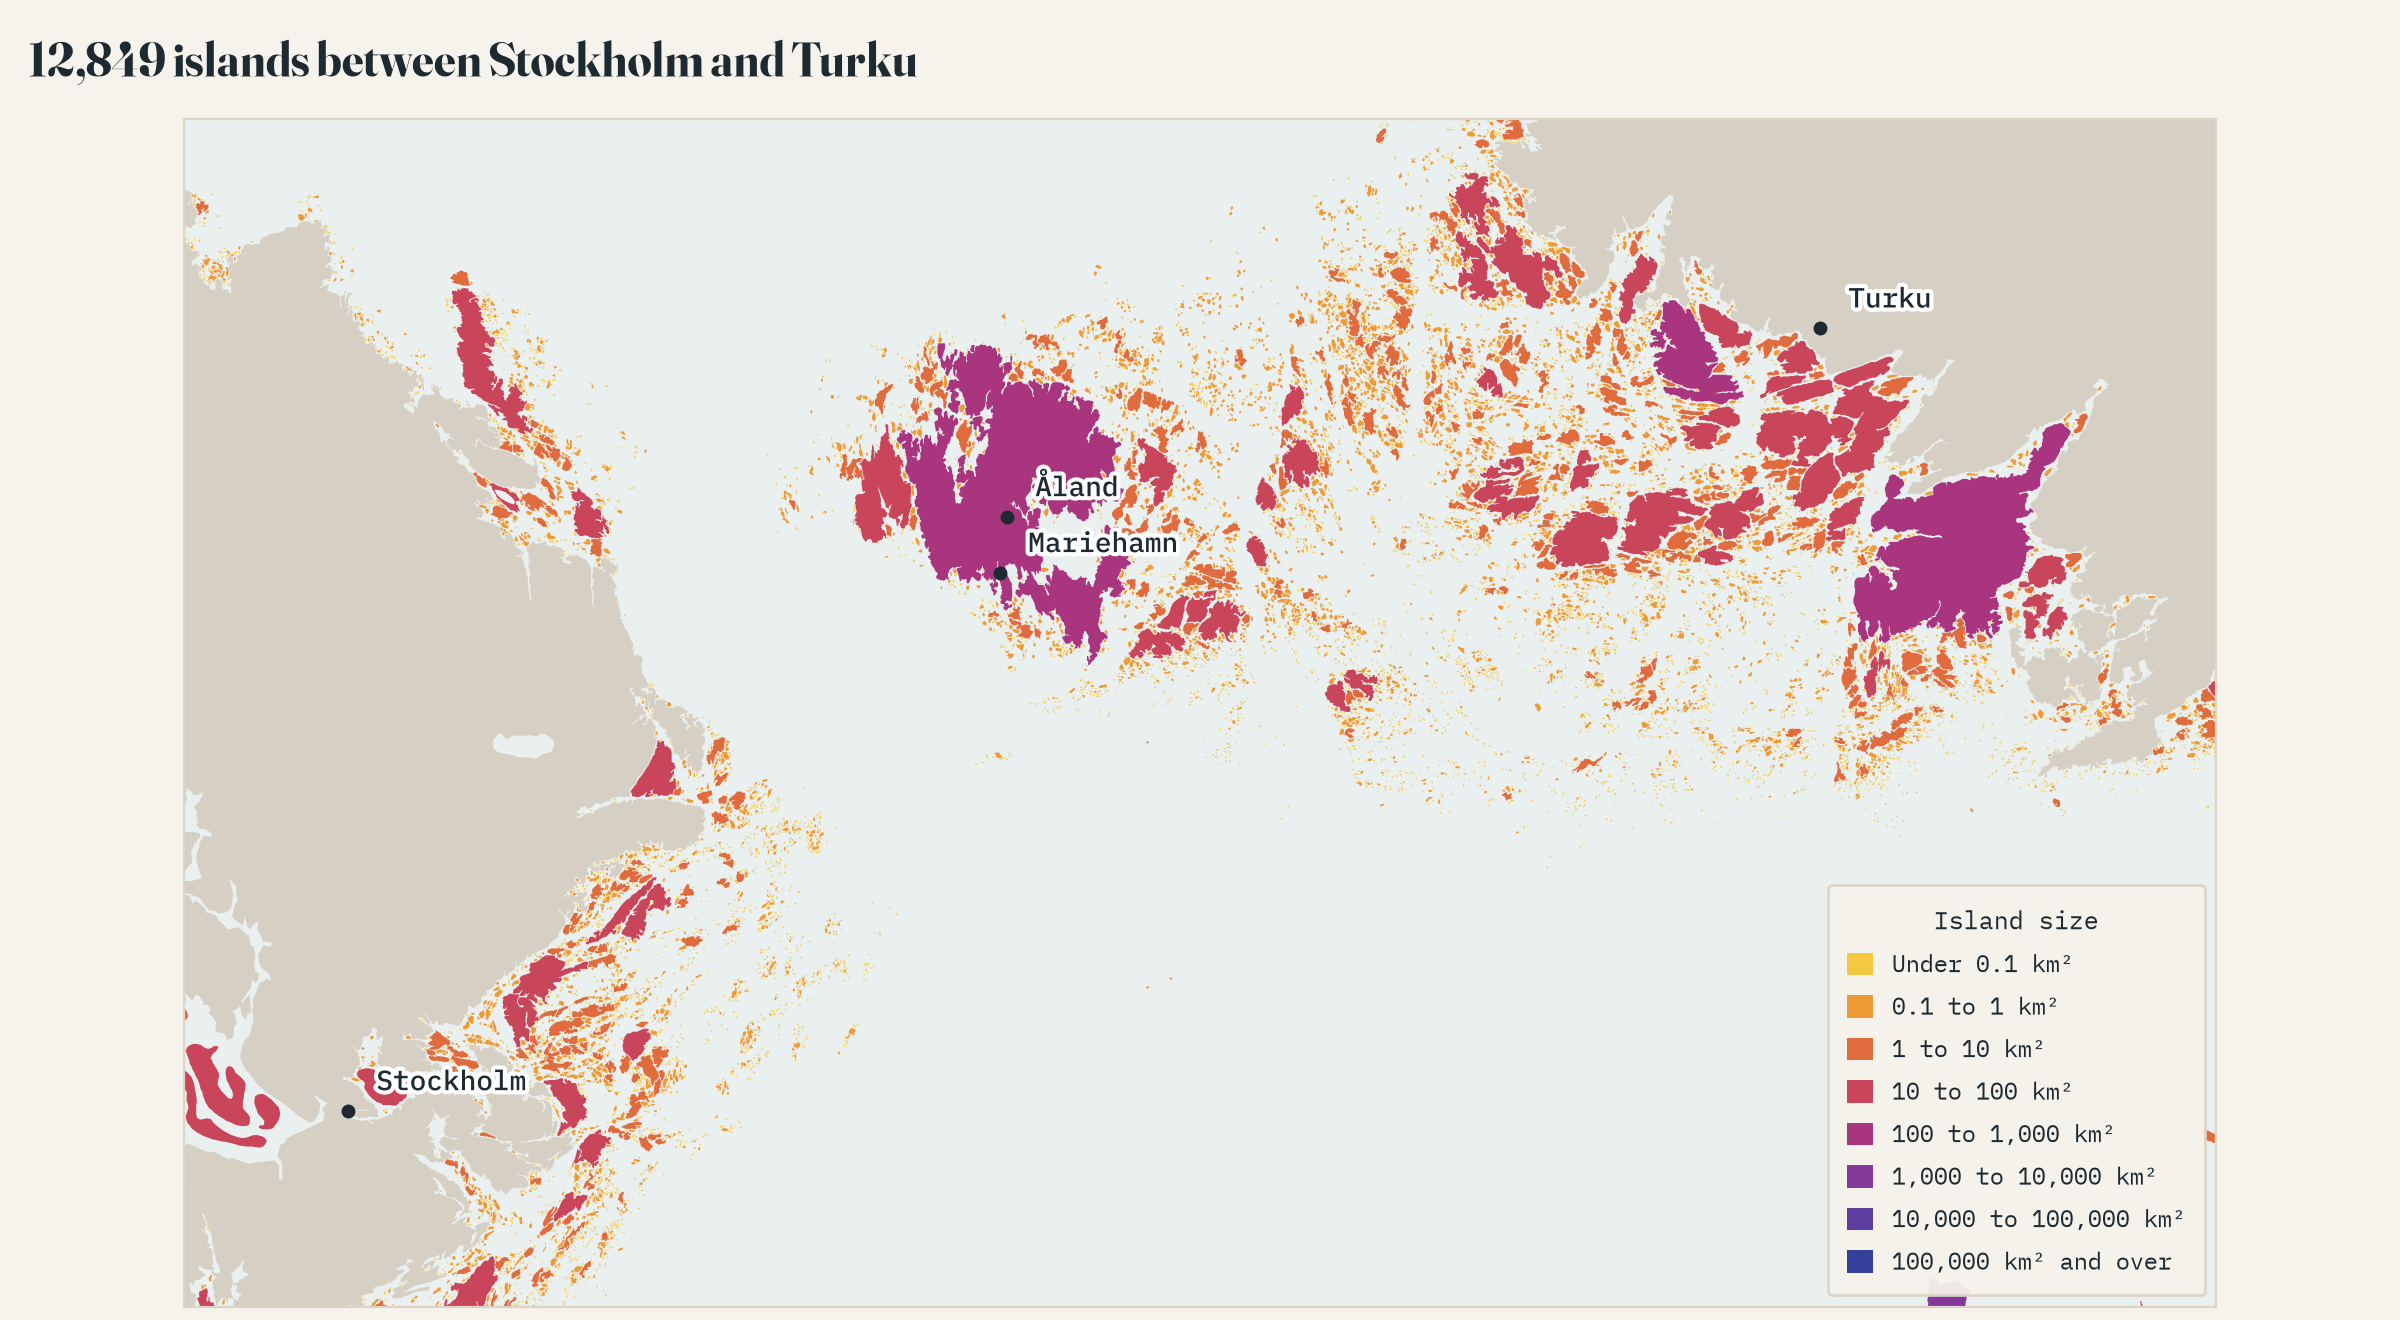
\includegraphics[width=\textwidth]{f_baltic.png}
\caption{The Stockholm archipelago, the {\AA}land islands and the Archipelago Sea in the full-resolution shoreline; mainland in grey.}\label{fig:baltic}\end{figure}

\subsection{Who has the islands}
Canada has the most islands at every threshold: 29,249 in all, 4,048 of 1 km$^2$ or more and 1,015 of 10 km$^2$ or more (Table~\ref{tab:cty}, Figure~\ref{fig:cty}). Counting all sizes, Greenland (18,222), Finland (13,178), the United States, Norway and Sweden follow, which reflects the many skerries of glaciated coasts. At 1 km$^2$ or more the order changes to the United States (1,652), Indonesia (1,544), Russia (1,438) and Chile (1,245). Sweden has 10,036 GSHHG islands, 467 of 1 km$^2$ or more, far from its national figure. Finland's GSHHG islands are almost all at sea (only 0.8\% in lakes), which shows how incomplete the shoreline is for the islands of Finland's lakes. With territories folded into their sovereign states, Denmark (with Greenland and the Faroes) has 18,490 islands.

\begin{table}[tbp]\centering\small\caption{Islands by country or territory (top 15 by islands of 1 km$^2$ or more), with island land area.}\label{tab:cty}\begin{tabular}{lrrrrr}\toprule Country or territory & All & 1+ km$^2$ & 10+ km$^2$ & 100+ km$^2$ & Area, km$^2$\\\midrule
Canada & 29,249 & 4,048 & 1,015 & 204 & 1,651,439\\
United States & 11,692 & 1,652 & 446 & 113 & 121,827\\
Indonesia & 6,836 & 1,544 & 472 & 143 & 1,698,962\\
Russia & 5,144 & 1,438 & 444 & 106 & 308,545\\
Chile & 8,046 & 1,245 & 393 & 118 & 129,014\\
Greenland & 18,222 & 1,153 & 336 & 69 & 2,165,772\\
Norway & 11,231 & 845 & 208 & 54 & 85,333\\
Australia & 5,864 & 794 & 179 & 37 & 97,357\\
Philippines & 3,383 & 591 & 177 & 46 & 297,003\\
Brazil & 1,907 & 556 & 206 & 51 & 64,814\\
Finland & 13,178 & 532 & 100 & 10 & 7,637\\
China & 3,631 & 500 & 114 & 13 & 42,089\\
Sweden & 10,036 & 467 & 68 & 3 & 8,581\\
Japan & 2,497 & 387 & 109 & 27 & 373,459\\
Papua New Guinea & 1,506 & 327 & 106 & 28 & 847,516\\
\bottomrule\end{tabular}\end{table}

\begin{figure}[tbp]\centering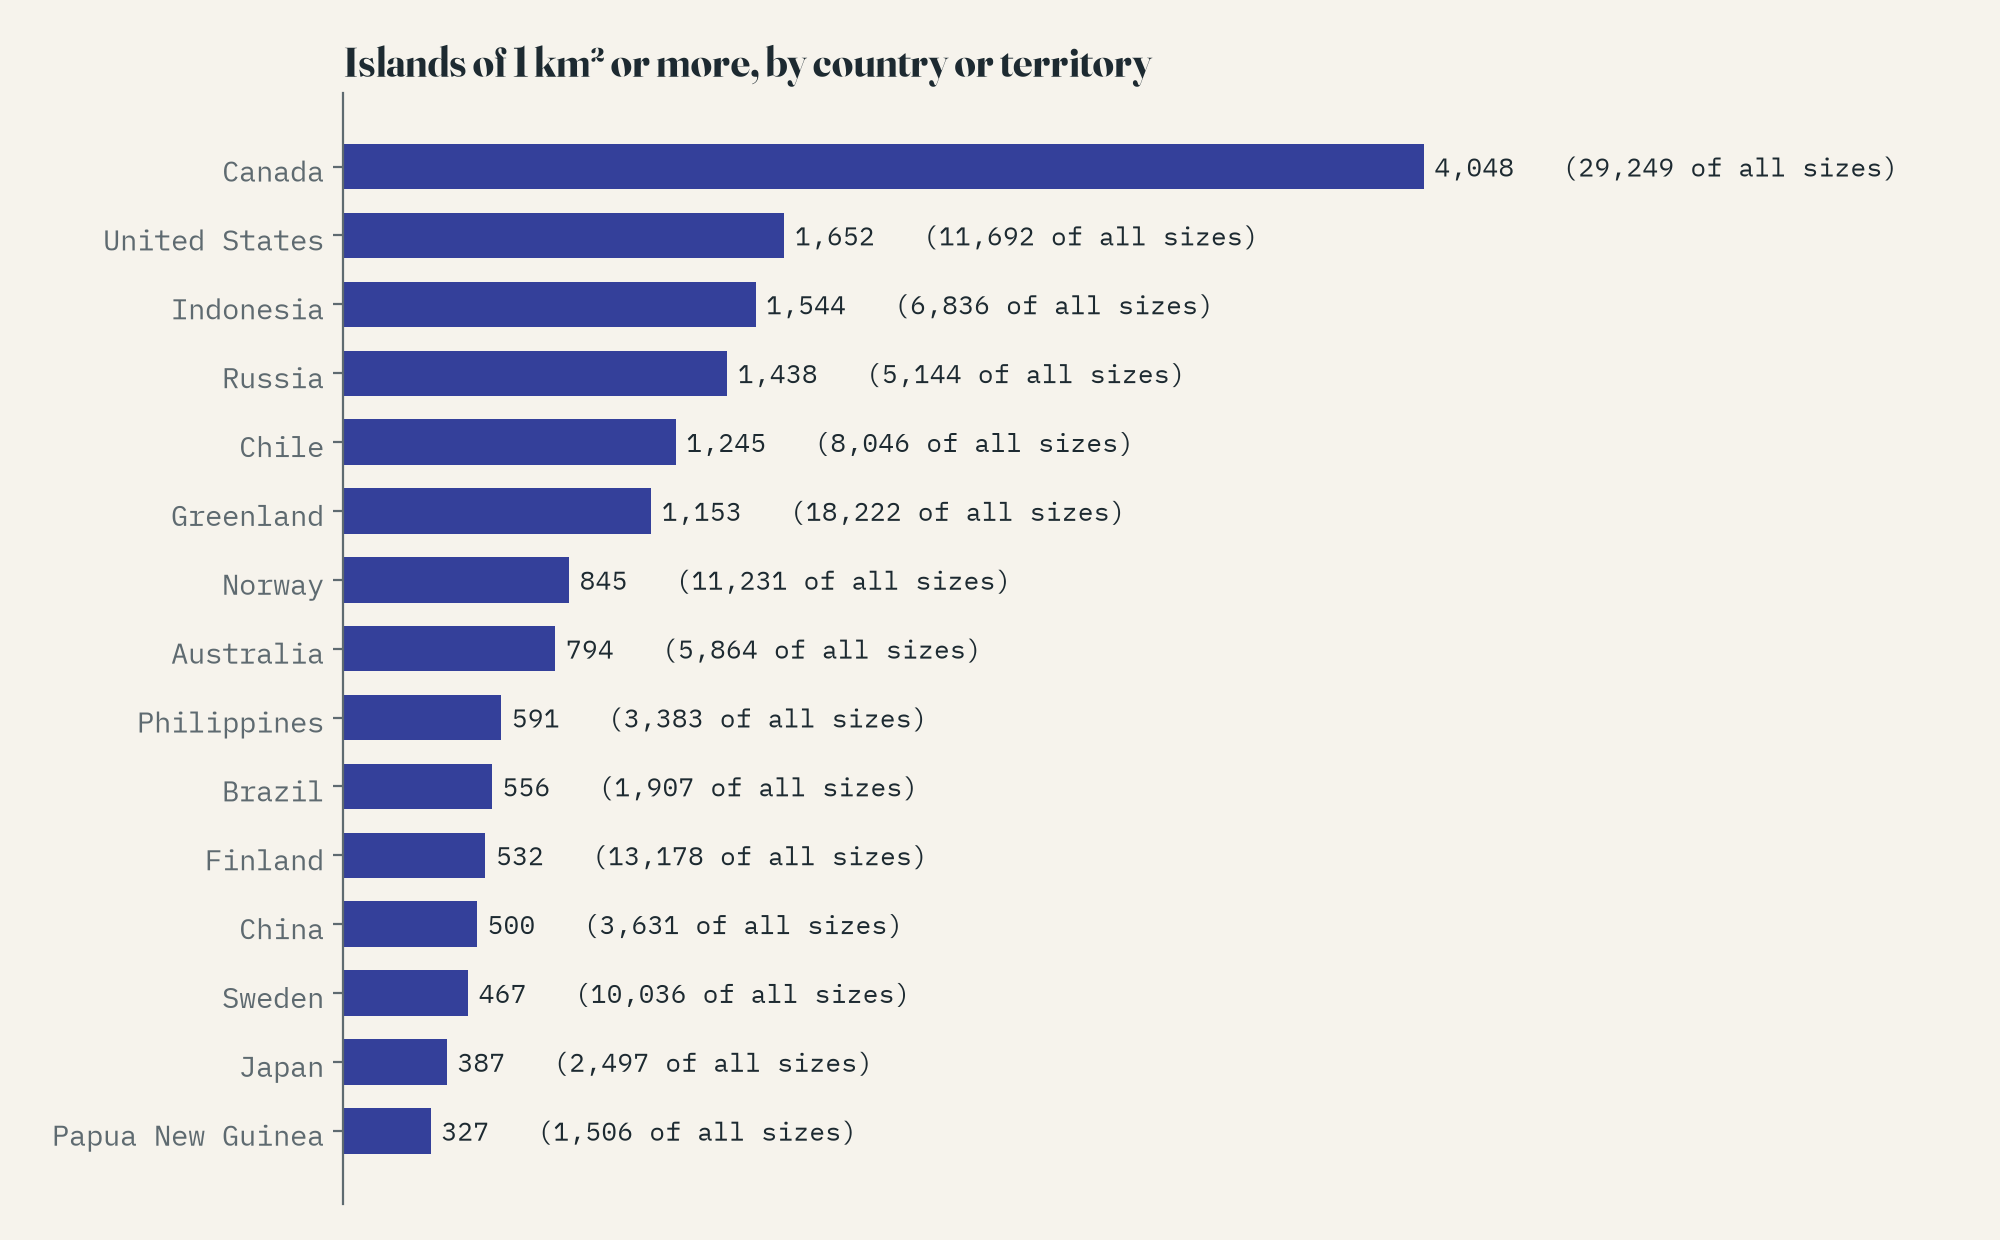
\includegraphics[width=0.92\textwidth]{f_countries.png}
\caption{Islands of 1 km$^2$ or more by country or territory (top 15), with the count of all sizes.}\label{fig:cty}\end{figure}

\subsection{The largest islands}
Greenland (2,113,828 km$^2$), New Guinea (780,025 km$^2$), Borneo (732,587 km$^2$), Madagascar, Baffin and Sumatra are the largest (Figure~\ref{fig:big}). Australia, at 3.6 times Greenland's area, is treated as a continent. Eight islands of over 1,000 km$^2$ are shared between countries in Natural Earth, among them New Guinea (Papua New Guinea 51.2\%, Indonesia 48.8\%), Borneo and Ireland. The largest islands in lakes are Manitoulin Island in Lake Huron (2,822 km$^2$) and Ren\'e-Levasseur Island in the Manicouagan Reservoir (2,012 km$^2$); the largest Antarctic island in this version of GSHHG is Adelaide Island (3,867 km$^2$), since islands bound into ice shelves, such as Alexander Island, are part of the Antarctic polygon.

\begin{figure}[tbp]\centering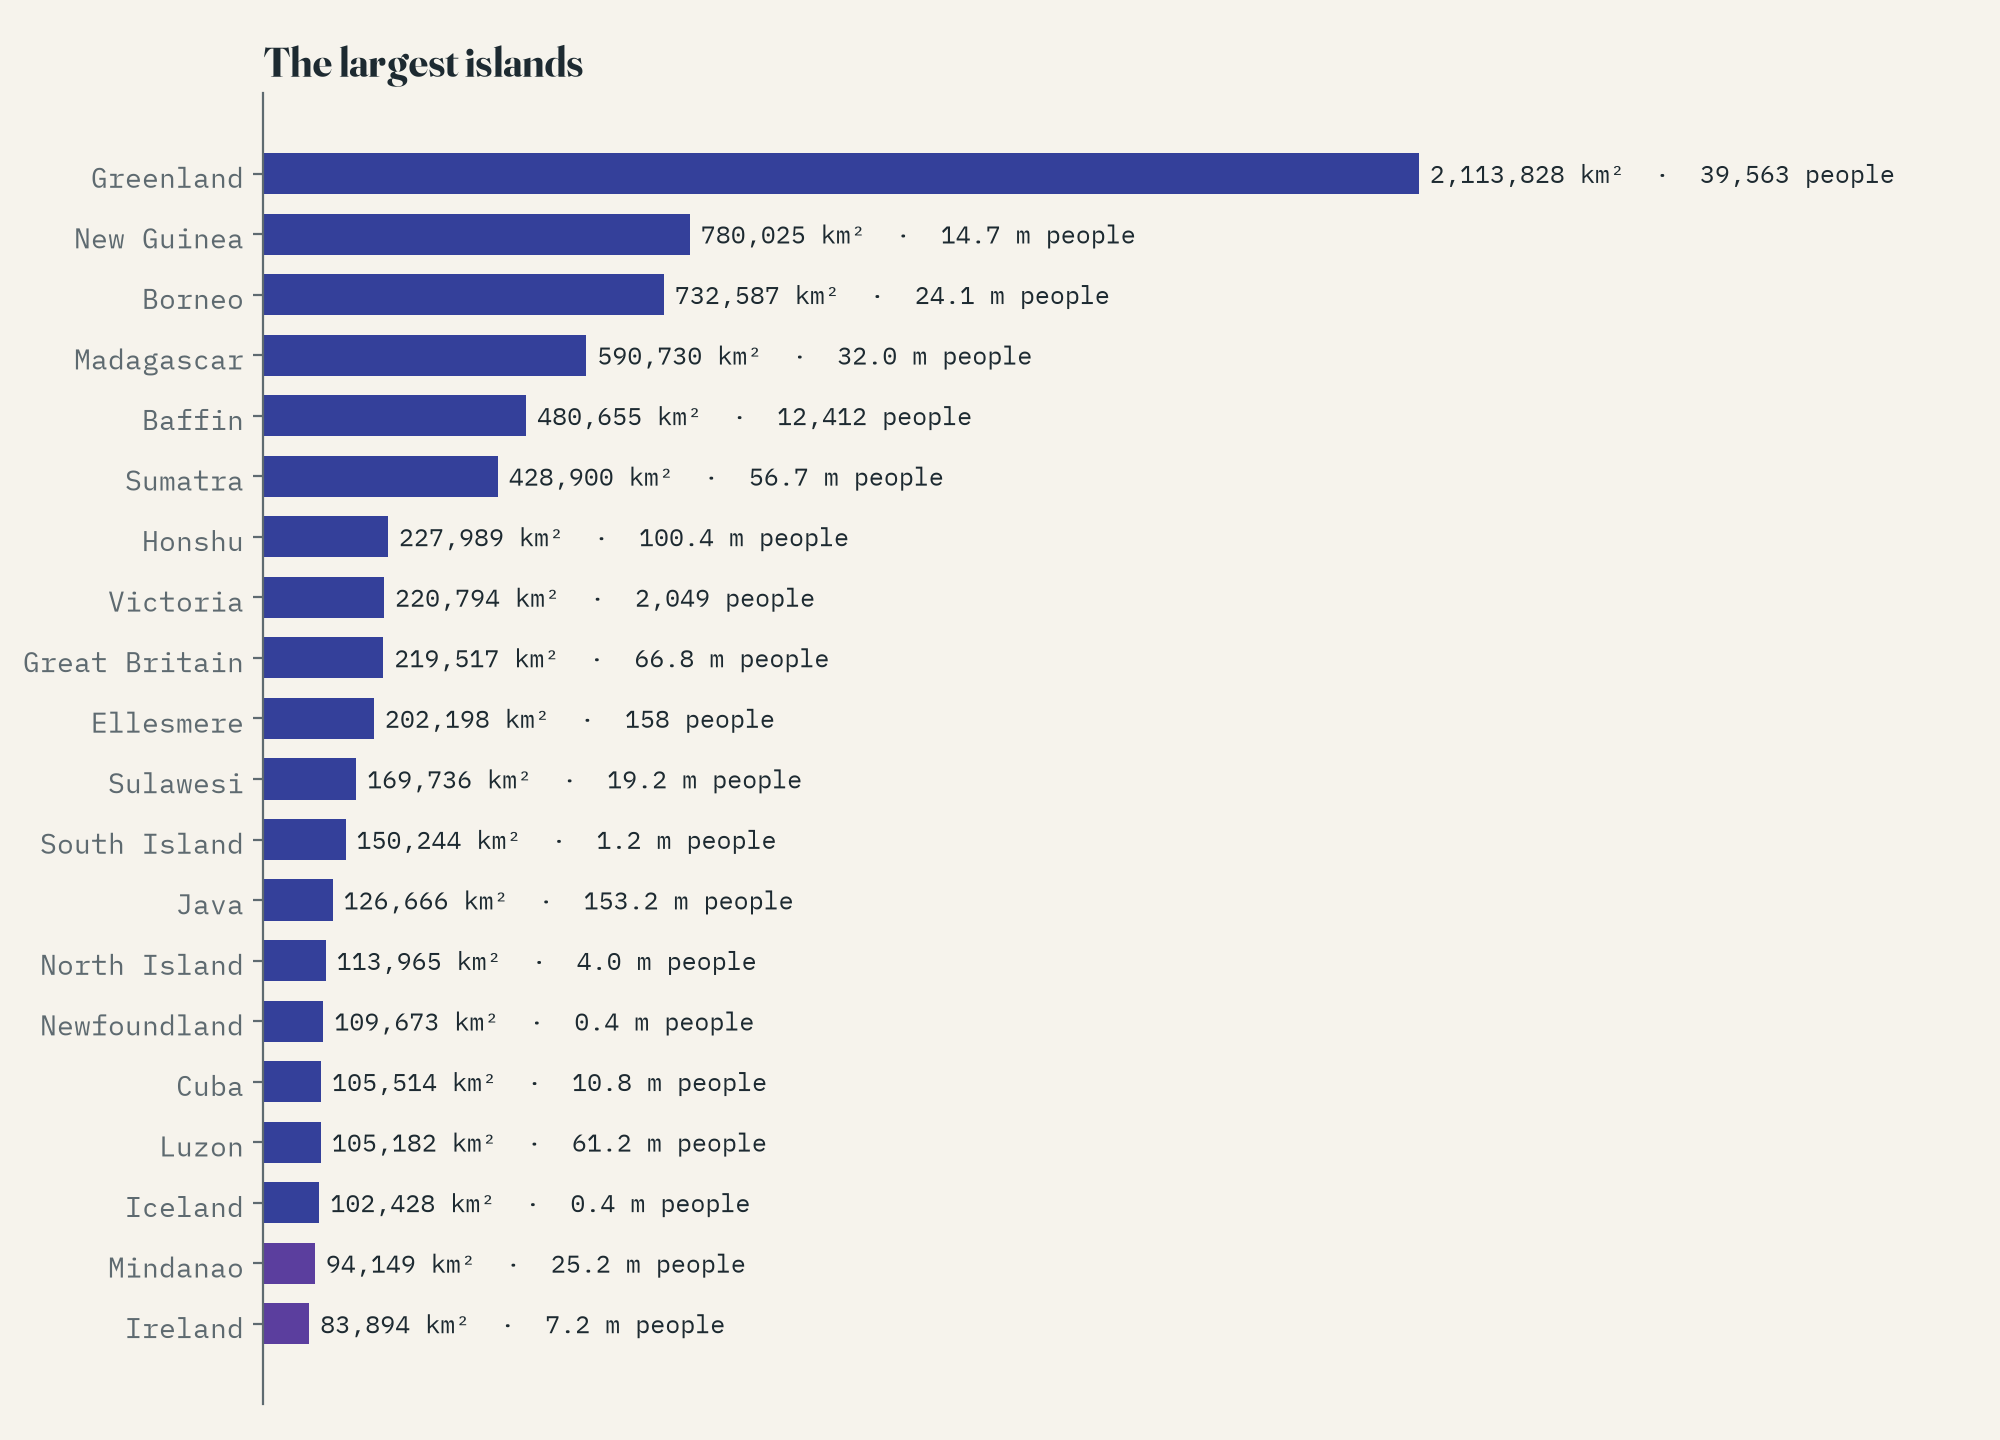
\includegraphics[width=0.92\textwidth]{f_largest.png}
\caption{The twenty largest islands, with their population in 2025.}\label{fig:big}\end{figure}

\subsection{People on islands}
Of the 8,187.6 million people in the WorldPop grid, 841.3 million (10.3\%) live on islands. They are concentrated on a few large islands (Figure~\ref{fig:pop}, Table~\ref{tab:pop}): Java has 153.2 million, 1.9\% of the world's population; Honshu 100.4 million and Great Britain 66.8 million. These three hold 38.1\% of island people, and the top ten 67.3\%. Islands of 10,000 km$^2$ or more hold 84.9\% of island people. 18,911 islands have anyone in the grid, 207 have 100,000 people or more and 55 have a million or more. Islands in lakes and rivers hold 6.0 million people, over half of them in Montreal and on the Mekong river island south of Phnom Penh.

By region, Asia's islands hold 614 million people (73.0\% of all island people), Europe's 93 million and Africa's 42 million. 43 countries and territories of 100,000 people or more have 99\% or more of their people on islands, together 754 million people. Among countries of over a million people with both island and mainland populations, the island share is highest in Denmark (56.3\%), Equatorial Guinea (28.5\%), Hong Kong (24.5\%) and Malaysia (21.1\%).

\begin{figure}[tbp]\centering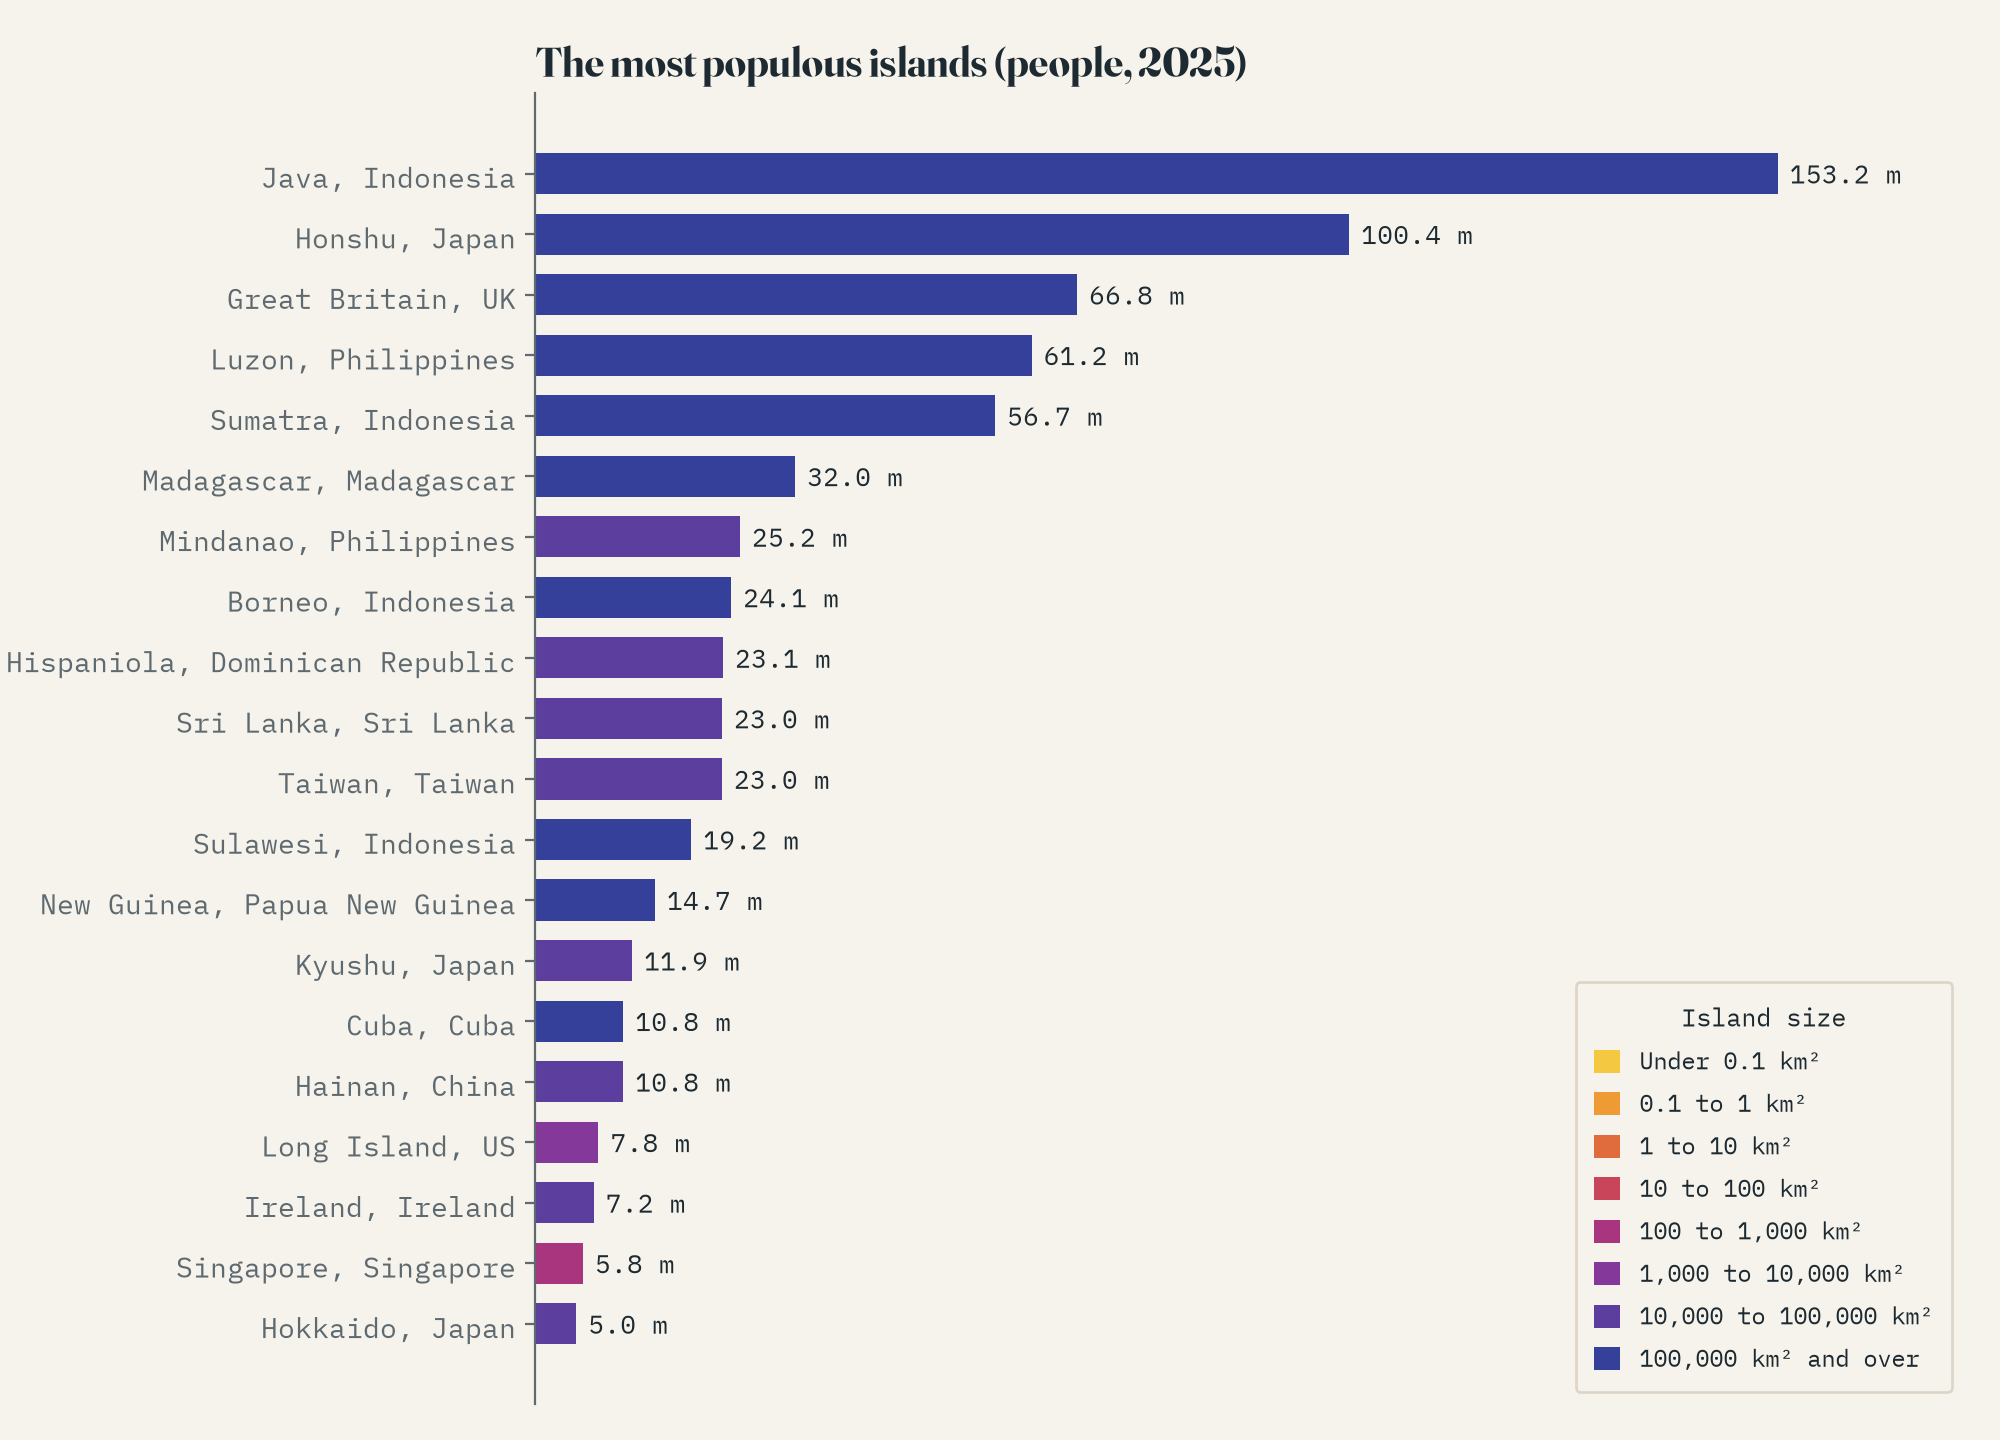
\includegraphics[width=0.92\textwidth]{f_populous.png}
\caption{The twenty most populous islands, WorldPop 2025, coloured by size class.}\label{fig:pop}\end{figure}

\begin{table}[tbp]\centering\footnotesize\caption{The 25 most populous islands, WorldPop 2025.}\label{tab:pop}\begin{tabular}{rllrrr}\toprule & Island & Country & Area, km$^2$ & People, m & Per km$^2$\\\midrule
1 & Java & Indonesia & 126,666 & 153.24 & 1,210\\
2 & Honshu & Japan & 227,989 & 100.37 & 440\\
3 & Great Britain & United Kingdom & 219,517 & 66.80 & 304\\
4 & Luzon & Philippines & 105,182 & 61.20 & 582\\
5 & Sumatra & Indonesia & 428,900 & 56.69 & 132\\
6 & Madagascar & Madagascar & 590,730 & 32.03 & 54\\
7 & Mindanao & Philippines & 94,149 & 25.22 & 268\\
8 & Borneo & Indonesia & 732,587 & 24.14 & 33\\
9 & Hispaniola & Dominican Republic & 74,316 & 23.13 & 311\\
10 & Sri Lanka & Sri Lanka & 65,799 & 23.00 & 350\\
11 & Taiwan & Taiwan & 35,818 & 22.99 & 642\\
12 & Sulawesi & Indonesia & 169,736 & 19.21 & 113\\
13 & New Guinea & Papua New Guinea & 780,025 & 14.74 & 19\\
14 & Kyushu & Japan & 36,927 & 11.91 & 323\\
15 & Cuba & Cuba & 105,514 & 10.82 & 103\\
16 & Hainan & China & 33,979 & 10.82 & 318\\
17 & Long Island & United States & 3,121 & 7.77 & 2,490\\
18 & Ireland & Ireland & 83,894 & 7.18 & 86\\
19 & Singapore & Singapore & 548 & 5.85 & 10,671\\
20 & Hokkaido & Japan & 77,813 & 5.02 & 65\\
21 & Negros & Philippines & 12,725 & 4.94 & 388\\
22 & Panay & Philippines & 11,484 & 4.68 & 408\\
23 & Sicily & Italy & 25,544 & 4.66 & 182\\
24 & Cebu & Philippines & 4,462 & 4.58 & 1,027\\
25 & Bali & Indonesia & 5,404 & 4.31 & 798\\
\bottomrule\end{tabular}\end{table}

\subsection{Crowded and empty islands}
Among islands of 100 km$^2$ or more, the most crowded is Xiamen Island (18,787 people per km$^2$), then Singapore (10,671), Montreal with Laval (3,511) and Staten Island (3,124) (Figure~\ref{fig:ce}). Among islands of 1,000 km$^2$ or more, Long Island is the most crowded (2,490), ahead of Java (1,210). Rankings of smaller islands are dominated by city districts on islets that the shoreline separates from their surroundings, where cells of 1 km cannot be trusted, so I do not report them. 77 islands of 1,000 km$^2$ or more have nobody in the grid, 67 of them in the Arctic or the far south; the largest is Devon Island (55,886 km$^2$). Uninhabited islands of every size make up 8.2\% of island land. Spitsbergen also appears empty, although Longyearbyen has a population of a few thousand: the constrained model places no one where its building layer finds no settlement.

\begin{figure}[tbp]\centering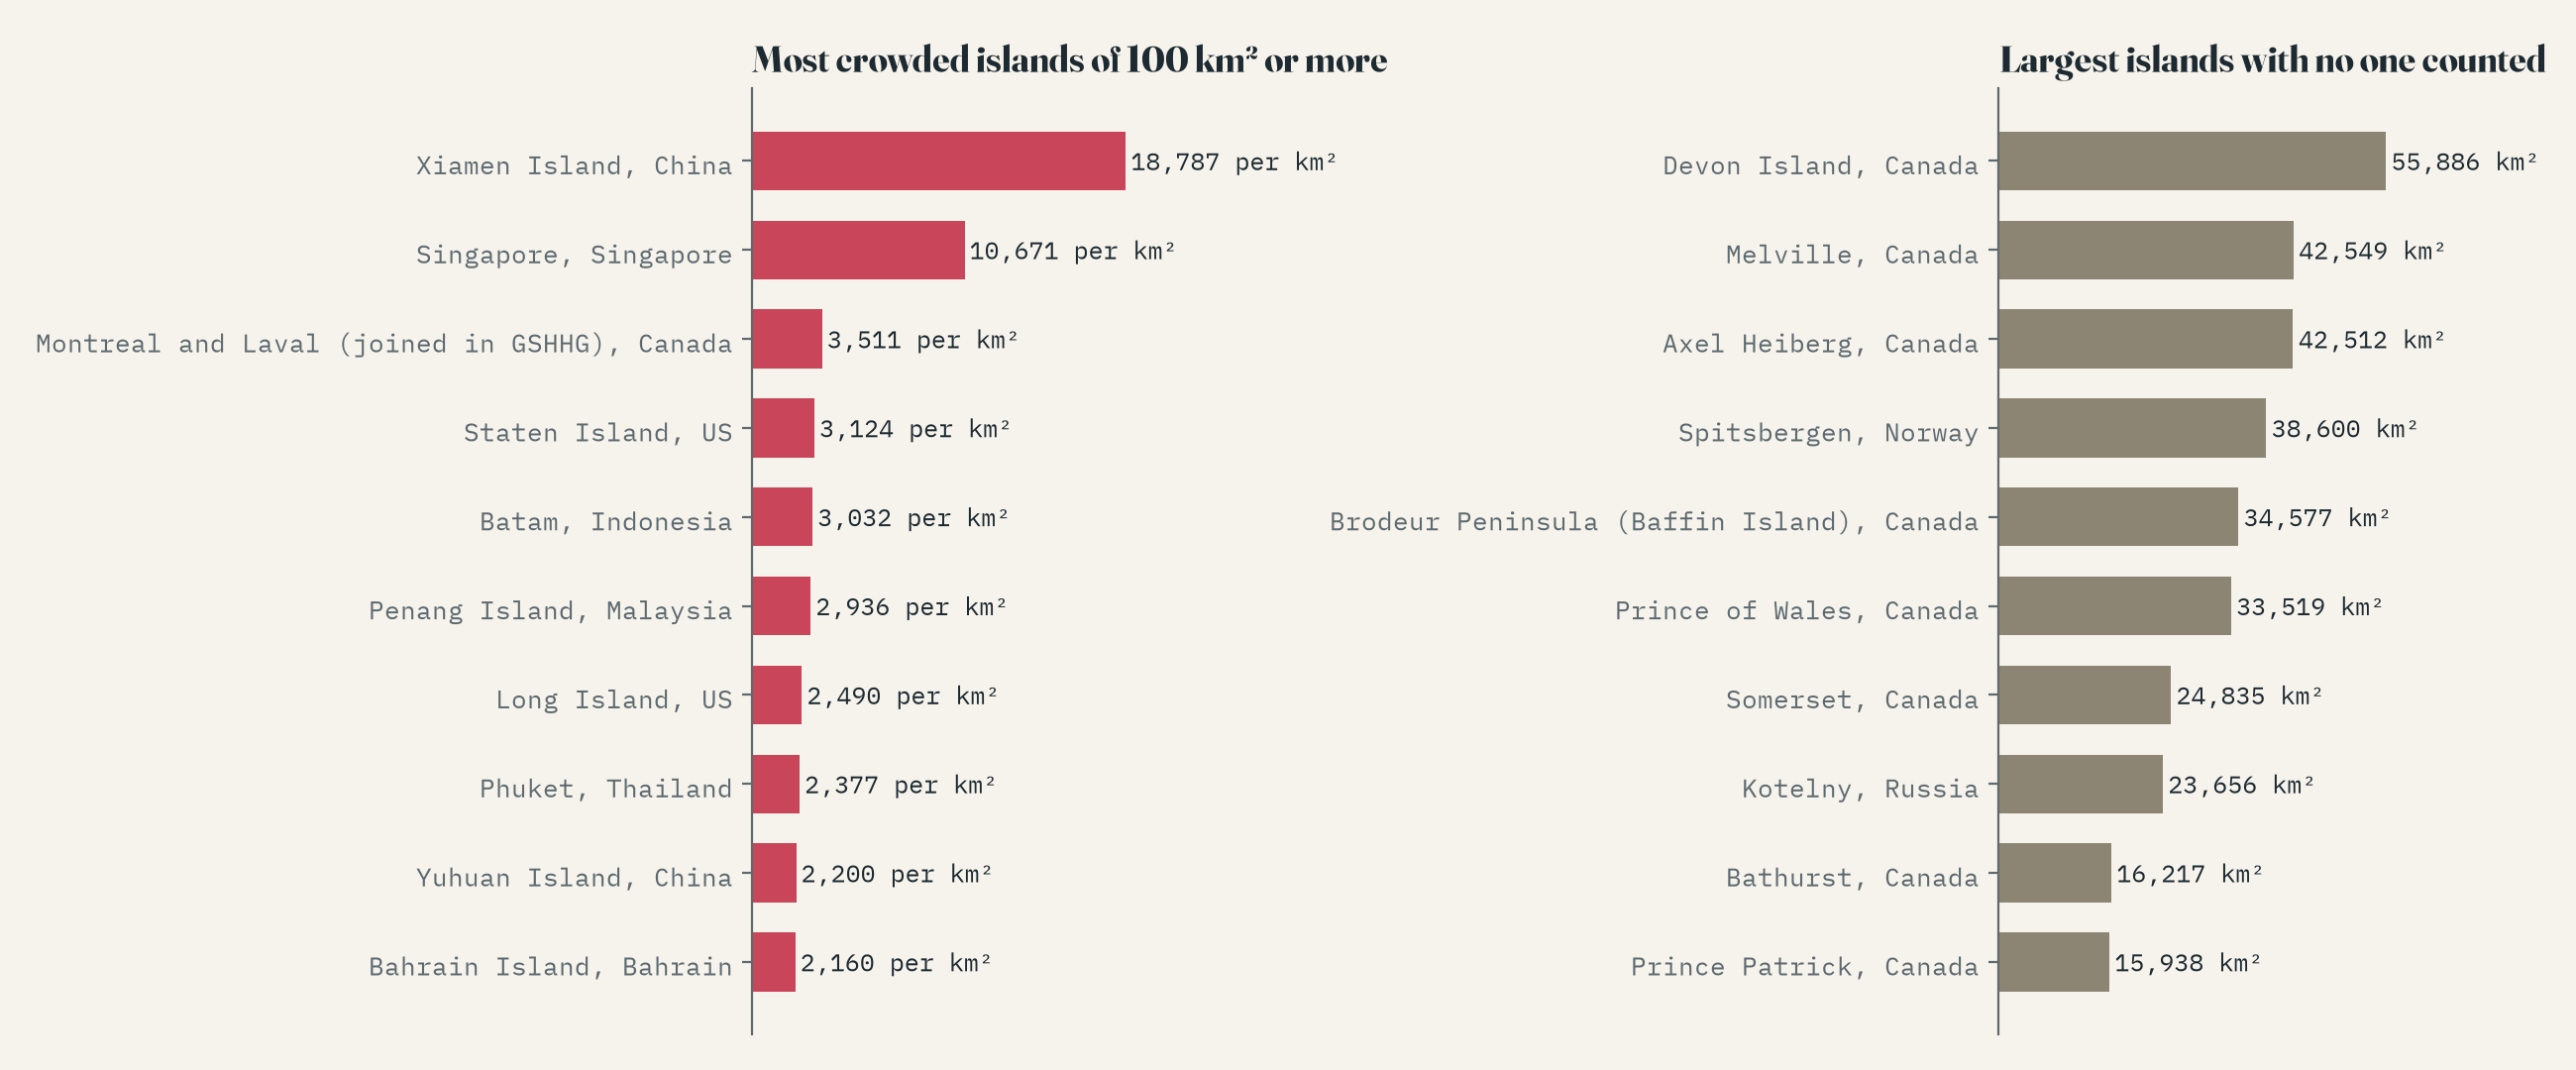
\includegraphics[width=\textwidth]{f_crowded_empty.png}
\caption{Left: people per km$^2$ on islands of 100 km$^2$ or more. Right: the largest islands with no one in WorldPop's 2025 grid.}\label{fig:ce}\end{figure}

\subsection{Islands in lakes on islands}
662 of GSHHG's 6,658 lakes lie on islands; the largest, at 3,141 km$^2$, is Amadjuak Lake on Baffin Island (Nettilling Lake, larger, is missing from the shoreline). 23 islands lie in lakes on islands (Figure~\ref{fig:nest}). The largest is Glover Island in Grand Lake, Newfoundland (163 km$^2$ in a lake of 632 km$^2$), followed by Talim Island in Laguna de Bay (28.2 km$^2$) and Volcano Island in Taal Lake (26.9 km$^2$), both on Luzon, and Isla Cabritos in Lake Enriquillo on Hispaniola (24.8 km$^2$). Samosir, often cited as the largest island in an island, is joined to the shore of Lake Toba in GSHHG. Deeper nesting, such as Vulcan Point in the crater lake of Volcano Island, is below the shoreline's hierarchy.

\begin{figure}[tbp]\centering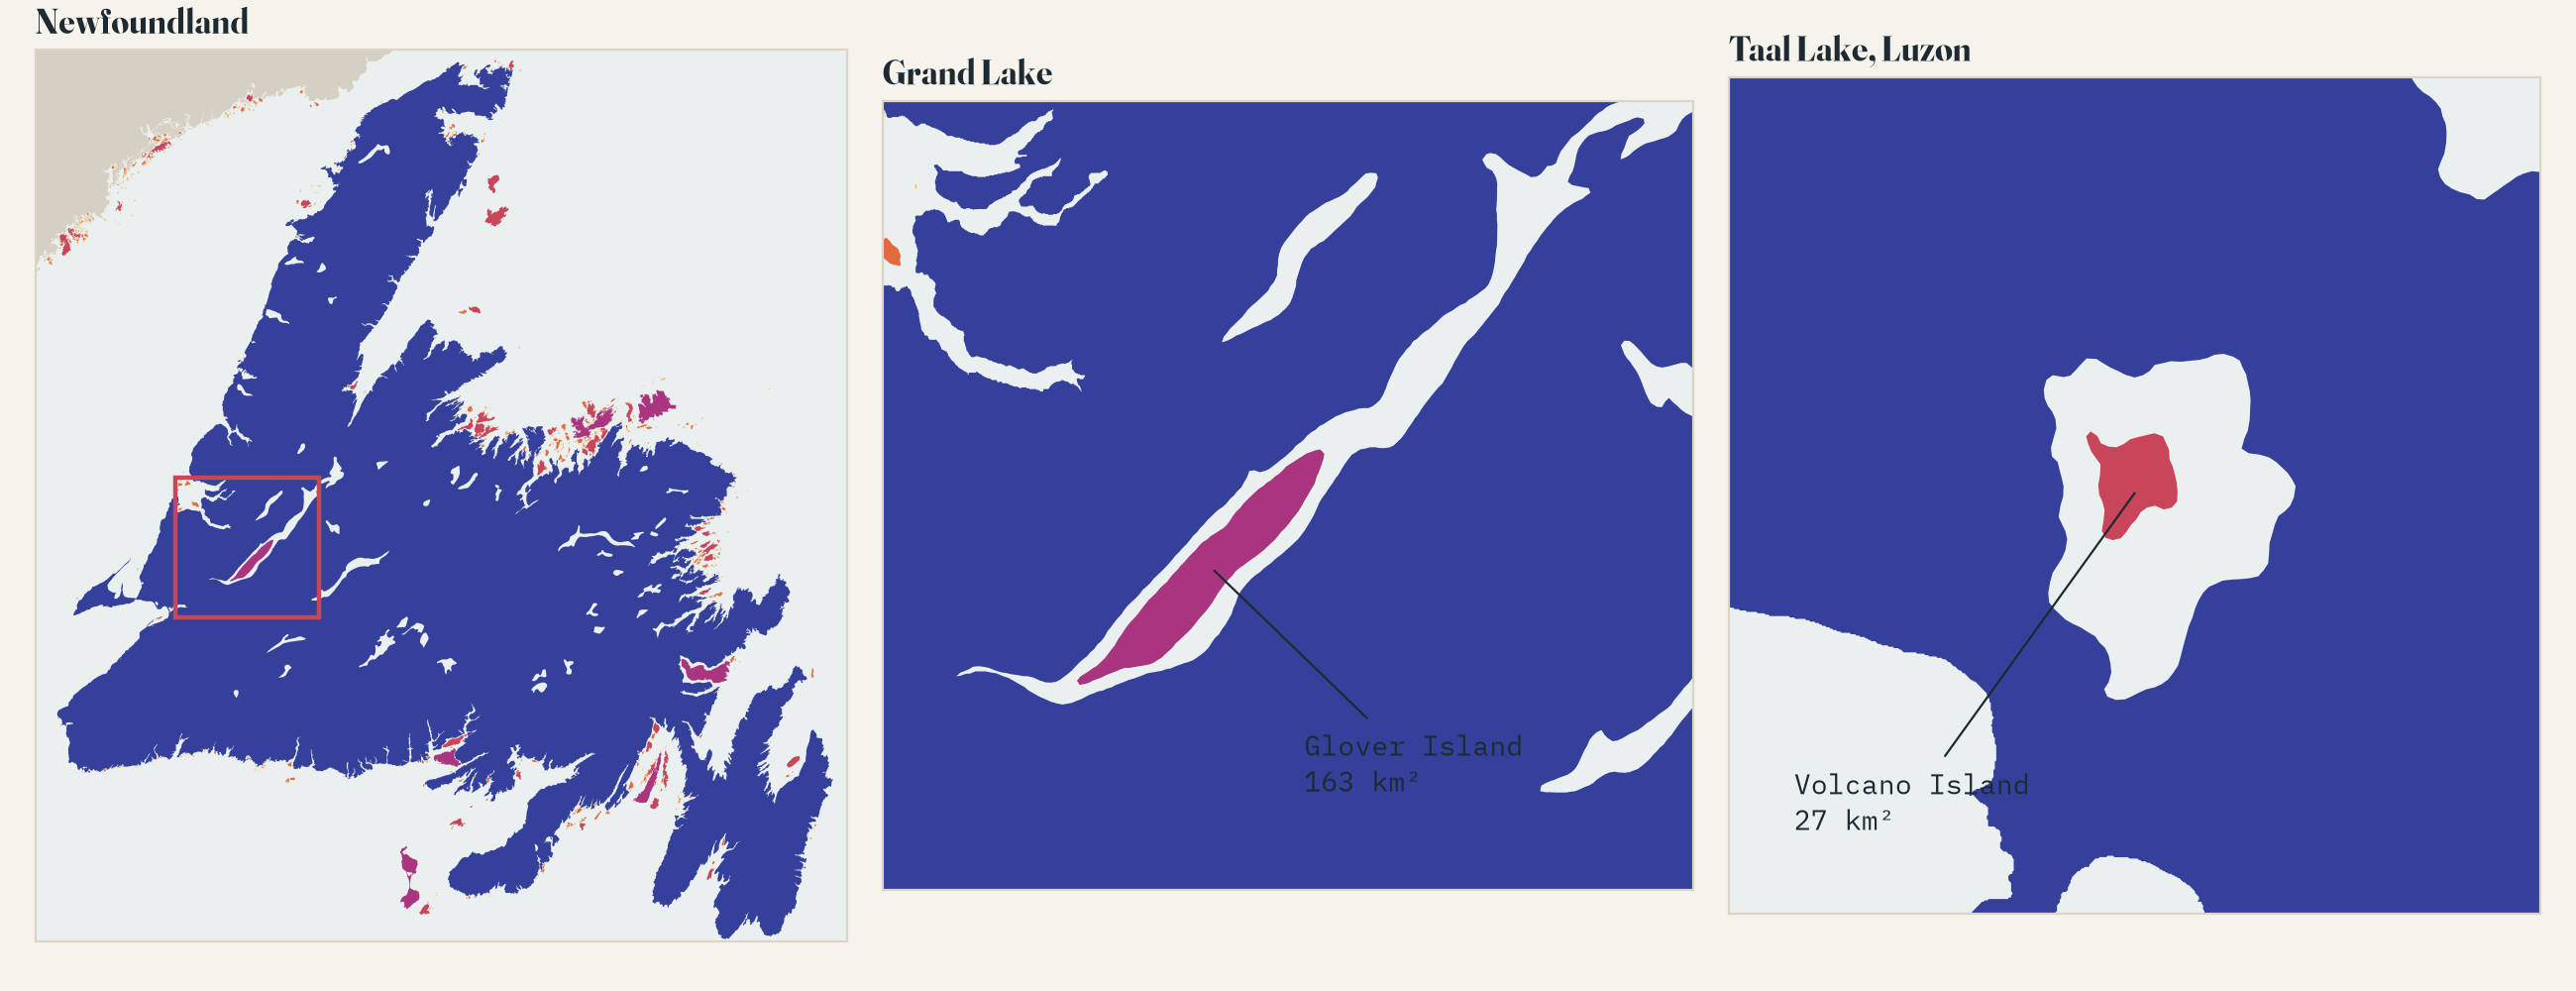
\includegraphics[width=\textwidth]{f_nested.png}
\caption{Islands in lakes on islands: Glover Island in Grand Lake, Newfoundland, and Volcano Island in Taal Lake, Luzon.}\label{fig:nest}\end{figure}

\section{Discussion}
The headline count of islands is a property of the map. A count that includes everything the full-resolution GSHHG draws is dominated by rocks and skerries under a tenth of a square kilometre, most of them on glaciated coasts, and more detailed national maps find many more. Counts of islands of a square kilometre or more are robust to resolution and are the sensible basis for comparison, on which Canada leads by a wide margin and the United States, Indonesia, Russia and Chile follow.

The human geography of islands is very different from their physical geography. A large part of island land is Arctic, and 8.2\% of it has no one in the grid, while island people are concentrated on a few large, fertile or urban islands in Asia and Europe. About one person in ten lives on an island. The figure depends on what the shoreline separates: if Manhattan and Salsette were islands in GSHHG, as they are in reality, it would rise; if Great Britain, Java and Honshu were treated as continents, as some definitions of an island might suggest for very large islands, it would fall sharply.

\section{Limitations}
First, resolution: GSHHG misses many small islands (especially in lakes and rivers, and in Finland's lakes in particular) and counts below 1 km$^2$ are not comparable with national counts. Second, shoreline judgements and age: GSHHG is built from older World Vector Shoreline and CIA World Data Bank data; it lacks recent reclamation, misses Nettilling Lake, joins some islands to neighbours or to the mainland and splits off the Brodeur Peninsula. Third, population: WorldPop is a model, its constrained version can miss small settlements and, at about 1 km, cannot divide people precisely across narrow channels. Fourth, attribution: countries follow Natural Earth's de facto borders, and big shared islands are assigned to the country with the largest share for counting, though national population totals use every cell. Fifth, names: island names are incomplete and some were added by hand.

\section{Conclusion}
The full-resolution GSHHG shoreline draws 181,588 islands, of which 23,150 are a square kilometre or more. They cover 6.6\% of the world's land and carry 10.3\% of its people. The data, code and an interactive map make it possible to look up any island and to repeat the count with other thresholds or shorelines.

\section*{Data and code availability}
The interactive map is at \url{https://maps.tristanhotham.com/world-islands/}. Data and code are at \url{https://github.com/Tristan-Hotham/world-islands} and archived with this paper at \url{https://doi.org/10.5281/zenodo.23848301}. Island outlines, tiles and points derived from GSHHG are LGPL-3.0; population figures derive from WorldPop (CC BY 4.0); Natural Earth is public domain; the derived tables and text are released under CC BY 4.0 and the code under the MIT licence.

\section*{AI statement}
I wrote the text, with drafting and editing assistance from Claude (Anthropic), which also helped prepare the analysis code. I reviewed and checked all text and results.

\begin{thebibliography}{9}
\bibitem[Mandelbrot(1967)]{mandelbrot} Mandelbrot, B. (1967) How long is the coast of Britain? Statistical self-similarity and fractional dimension. \emph{Science}, 156(3775), 636 to 638.
\bibitem[Natural Earth(2026)]{naturalearth} Natural Earth (2026) Admin 0 countries, physical labels, land, minor islands and populated places (1:10m). Public domain. \url{https://www.naturalearthdata.com/}
\bibitem[Wessel and Smith(1996)]{gshhg} Wessel, P. and Smith, W. H. F. (1996) A global, self-consistent, hierarchical, high-resolution shoreline database. \emph{Journal of Geophysical Research}, 101(B4), 8741 to 8743.
\bibitem[WorldPop(2024)]{worldpop} WorldPop (2024) Global 2 population estimates, release 2024B, constrained, 2015 to 2030, 30 arc seconds. School of Geography and Environmental Science, University of Southampton. CC BY 4.0. \url{https://www.worldpop.org/}
\end{thebibliography}
\end{document}
